\chapter{Implementación}

Para la implementación de la solución utilizaremos una arquitectura cliente-servidor\cite{client-server}, la cual nos
permite tener los datos centralizados en una aplicación servidor. La aplicación cliente realizará peticiones al
servidor, para que este le provea de los datos que necesite en cada momento.\\

\section{Servidor}
En el lado del servidor o \textit{back-end} se encuentra la mayor parte de la lógica de la aplicación, dedicándose el
lado del cliente a simplemente mostrarla en una interfaz cómoda para el usuario.\\

Se ha implementado un servidor que provee a los clientes de un listado de series y sus temporadas, así como de la
posibilidad de crear reseñas de las mismas o obtener las reseñas de otros usuarios.

\subsection{Lenguaje de programación}
El lenguaje de programación seleccionado para el servidor es \textit{Python}\cite{python}, ya que es un lenguaje de programación que
nos provee de una buena experiencia de desarrollo al ser un lenguaje menos estricto y cuenta con muchas librería útiles
y una enorme comunidad a sus espaldas.\\

Uno de sus puntos débiles, es que al ser un lenguaje no tipado, es más propenso a errores de sintaxis, pero desde la
versión 3.5, cuenta con una forma de tipar el código, de forma que, aunque el intérprete de \textit{Python} no detecte
este tipado, puede ser utilizado por herramientas de los \textit{IDEs} y \textit{linters} para la detección precoz
errores.\\

Otro de los motivos que me han llevado a decantarme por este lenguaje son sus librerías científicas y de procesamiento
de datos. Con ellas, en un futuro podríamos incluir en la aplicación alguna herramienta para obtener estadísticas y
realizar predicciones sobre nuestros datos. Algo muy útil para un cliente que quiera usar los datos de la aplicación
para saber qué tipo de series interesan a cierto tipo de público, por ejemplo.\\

Como gestor de paquetes y dependencias, utilizo \textit{poetry}\cite{poetry}, que nos permite gestionar las dependencias del proyecto
de forma muy sencilla y similar a \textit{NPM}\cite{npm}.

\subsection{Test}
Como ya hablamos en la \hyperref[chap:metodología]{metodología}, necesitamos que el código cumpla con unos requisitos
mínimos de calidad a través de \textit{tests}.\\

Para el servidor, se han implementado tests unitarios con la librería \textit{pytest}\cite{pytest}, que comprueban que los métodos de
los modelos de la aplicación funcionan correctamente.
\begin{figure}[H]
\centering	
    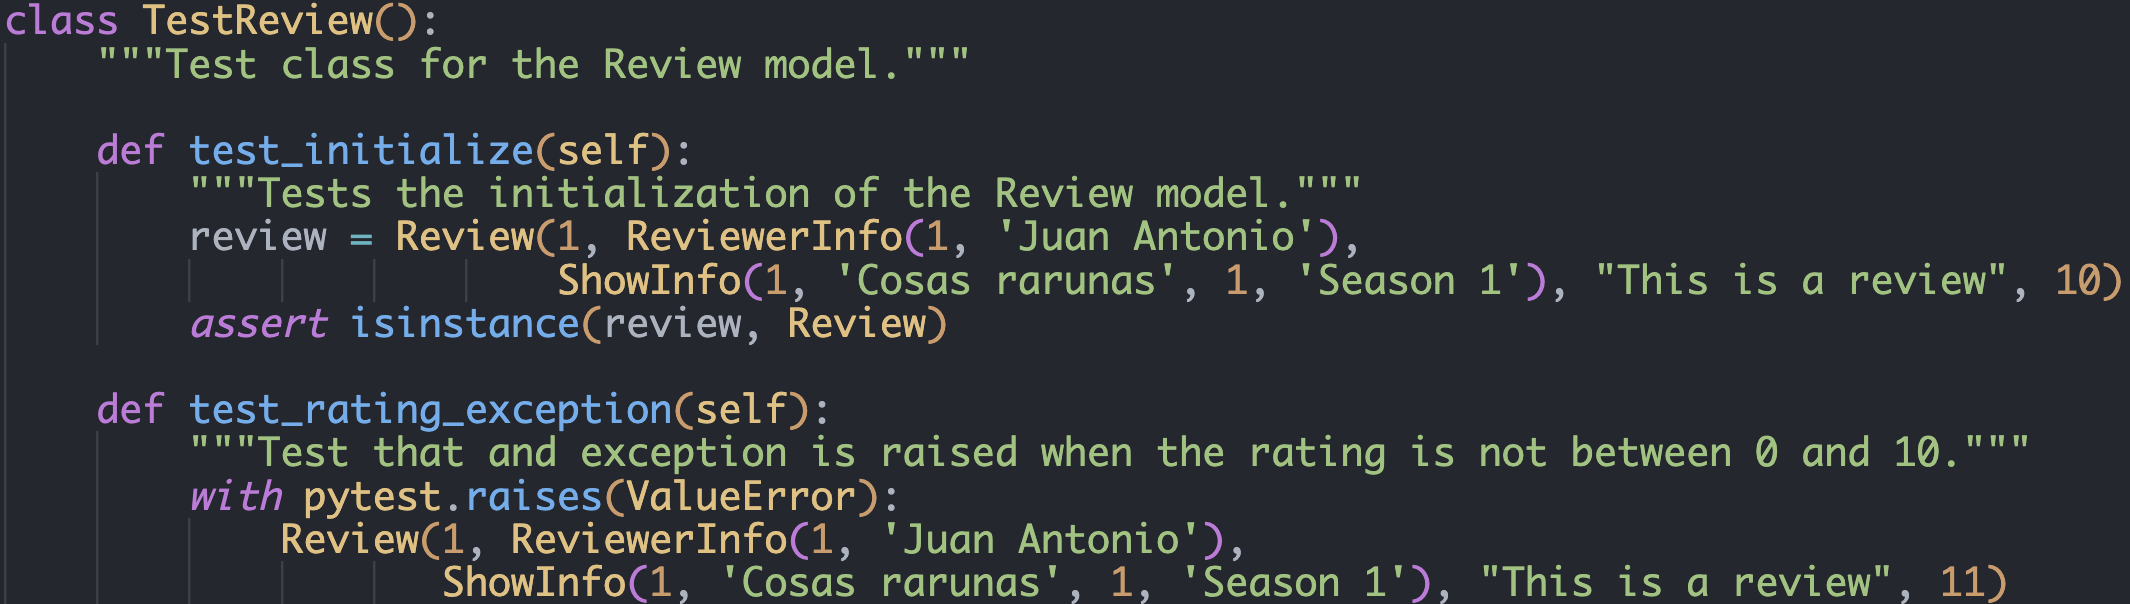
\includegraphics[scale=0.25]{img/pytest.png}
\caption{ Test unitario de la clase Show en Python }\label{fig:pytest}
\end{figure}
